\documentclass[
		12pt,
		a4paper,
		toc=listof, %% Abbildungs- und Tabellenverzeichnis mit ins Inhaltsverzeichnis
		bibliography=totoc %% Quellenverzeichnis mit ins Inhaltsverzeichnis
		]{scrreprt}	 %% KOMA Script

% HTWG
\usepackage{graphicx}
\usepackage{a4}
\usepackage{german}

% Eigene
\usepackage[utf8]{inputenc} %% Umlaute
\usepackage[printonlyused, withpage]{acronym} %% Abkuerzungsverzeichnis (nur verwendete)
\usepackage{todonotes} %% TODOs moeglich mit \todo{}
\usepackage{booktabs} %% Tabellen
\usepackage{amsmath} %% Formeln
\usepackage{listings} %% Codebeispiele
\usepackage{subfigure} %% Mehrere Bilder nebeneinander
\usepackage{hyperref} %% referenzen innerhalb und außerhalb des Dokumentes
\usepackage[headsepline]{scrpage2} %%Numerrierung der Seiten + Kapitelnamen in Kopfzeile inkl. Trennstrich
\pagestyle{scrheadings} %% die folgenden Zeilen sorgen für die korrekte Nummerierung und deren Anzeige 
\clearscrheadfoot %% und für die Kopfzeile mit aktuellem Kapitel etc.
\ihead{\headmark}
\cfoot[\pagemark]{\pagemark}
\automark{chapter}
\usepackage{float} %% Floatpackage um Grafik-Positionen zu forcieren
\newcommand*{\quelle}[1]{\par\raggedleft\footnotesize Quelle:~#1}
\usepackage{textcomp}
\usepackage{eurosym}
\usepackage{graphicx}

% Eigenes Design 
%TODO loeschen wenn default HTWG Design (was es nicht wirklich gibt) gewuuenscht ist
\usepackage[bottom=3cm]{geometry}
\usepackage{setspace}
\onehalfspacing


% KOMA script anpassungen 
%TODO entfernen wenn kein KOMA Script gewuenscht
\usepackage{scrhack}

%%%%%%%% Codebeispiele
\usepackage{color}
\usepackage{xcolor}
\usepackage{listings}
\usepackage{caption}

\setcounter{tocdepth}{2}  %% Uebreschriften bis subsectionw ins Inhaltsverzeichnis
\setcounter{secnumdepth}{3}  %% Nummerierung bis subsection


%%% Codebeispiele - Style
\DeclareCaptionFont{white}{\color{white}}
\DeclareCaptionFormat{listing}{\colorbox{gray}{\parbox{\textwidth}{#1#2#3}}}
\captionsetup[lstlisting]{format=listing,labelfont=white,textfont=white}

% Entfernt Kapitel Ueberschrift
% Bsp.
% 	ALT:
%       Kapitel 1
%       Einführung
%
% 	NEU:
% 		1 Einführung
%
\renewcommand*\chapterheadstartvskip{\vspace{-\topskip}}
\newcommand{\thema}{Bachelor-Thesis}
\newcommand{\forschungsfrage}{Thesis Thema}
\newcommand{\ausgabedatum}{Ausgabedatum}
\newcommand{\abgabedatum}{Abgabedatum}
\newcommand{\autor}{Max Mustermann}
\newcommand{\matrikelnummer}{123456}
\newcommand{\unternehmensbetreuer}{Unternehmensbetreuer}
\newcommand{\erstbetreuer}{Erstbetreuer}
\newcommand{\firma}{Unternehmen}
\newcommand{\studiengang}{Studiengang}
\newcommand{\autorGeburtsdatum}{Geburtsdatum}
\newcommand{\autorGeburtsort}{Geburtsort}



\begin{document}
%% Nummerierung aus
\pagenumbering{gobble}

% HTWG Templates fuer Titelseite etc.

\begin{titlepage}

\vspace*{-3.5cm}

\begin{center}

\includegraphics[width=5cm]{htwg/htwg-logo}

Fakultät Informatik \\
Fachbereich Wirtschaftsinformatik
\end{center}

\vspace*{1cm}

\begin{center}
	\huge{
		\textbf{\thema} \\[1cm]
	}
	\normalsize{
		\textbf{\forschungsfrage} \\[2cm]
	}
\end{center}
\begin{tabular}{p{6cm}p{8cm}}
                 \bfseries{Name:} & \autor \\[0.4cm]
                 \bfseries{Matrikelnummer:} & \matrikelnummer \\[0.4cm]
                 \bfseries{Unternehmen:} & \firma  \\[0.4cm]
                 \bfseries{Unternehmensbetreuer:} & \unternehmensbetreuer \\[0.4cm]
                 \bfseries{Erstkorrektor:} & \erstbetreuer \\[0.4cm]
                 \bfseries{Abgabetermin:} & \abgabedatum \\[0.4cm]
\end{tabular}
\\[1cm]
\begin{flushright}
	Konstanz, \abgabedatum \\
	Der Vorsitzende des Prüfungsausschusses \\[1.5cm]
	Prof. Dr. Renato Dambe
\end{flushright}
\end{titlepage}
\pagenumbering{Roman}
\addchap{Ehrenw"ortliche Erkl"arung}


Hiermit erkl"are ich
\textit{\autor, geboren am \autorGeburtsdatum{} in \autorGeburtsort{}},\\

\begin{tabular}{lp{12cm}}
(1) & dass ich meine Bachelorarbeit mit dem Titel: \\[1em]
& \textbf{\forschungsfrage} \\[1em]
& bei der \firma\ unter Anleitung von \erstbetreuer\ selbst"andig und ohne fremde Hilfe angefertigt habe und keine anderen als die angef"uhrten Hilfen benutzt habe;\\[1em]
(2) & dass ich die "Ubernahme w"ortlicher Zitate, von Tabellen, Zeichnungen, Bildern und
Programmen aus der Literatur oder anderen Quellen (Internet) sowie die Verwendung
der Gedanken anderer Autoren an den entsprechenden Stellen innerhalb der Arbeit
gekennzeichnet habe.\\
(3) & dass die eingerichten Abgabe-Exemplare in Papierform und im PDF-Format vollständig übereinstimmen.
\end{tabular}

\vspace*{1cm}

\noindent
Ich bin mir bewusst, dass eine falsche Erkl"arung rechtliche Folgen haben wird.\\

\vspace*{3cm}

\noindent
Konstanz, \abgabedatum \hfill \begin{tabular}{c} \\ \\ \rule{5cm}{1pt} \\ (Unterschrift)\end{tabular}

\tableofcontents
\addcontentsline{toc}{chapter}{Inhaltsverzeichnis}
\addchap{Abkürzungsverzeichnis}

\begin{acronym}[BPMN]
\acro{api}[API]{Application programming interface}
\acro{http}[HTTP]{Hypertext Transfer Protocol}
\acro{ssh}[SSH]{Secure Shell}
\end{acronym}


\clearpage
%% Starte Paginierung
\pagenumbering{arabic}

\include{kapitel1/Einleitung}

\chapter{Grundlagen}
\section{Abschnitt} 
\subsection{Unterabschnitt}
\begin{figure}
\makebox[\textwidth]{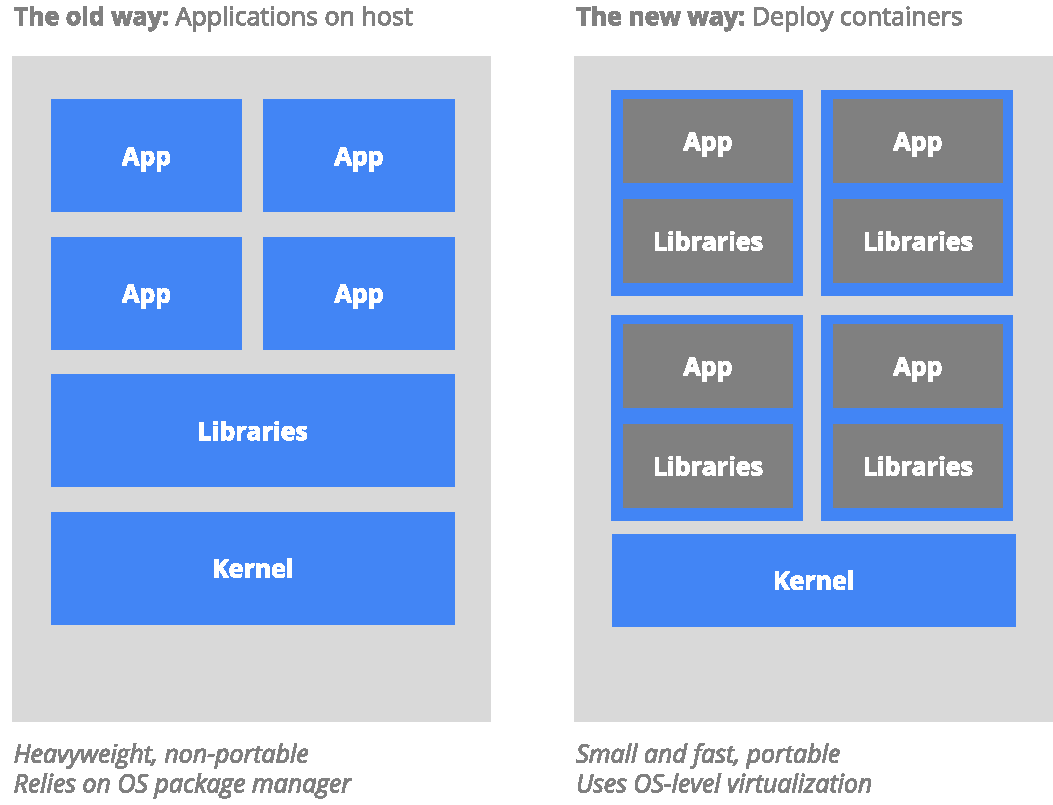
\includegraphics[width=\linewidth]{kapitel2/images/Platzhalter}}
\caption{Bildunterschrift}
\quelle\url{https://tinyurl.com/k3q2n7u} 
\label{Grundlagen:LabelDesPlatzhalters}
\end{figure}

Hier ist ein beispielhafter Verweis auf das Bild: \ref{Grundlagen:LabelDesPlatzhalters} 
Hierfür zitieren wir noch \cite{Anderson.2015}

\chapter{Konzept}



\chapter{Implementierung}


\chapter{Evaluation}


\chapter{Fazit und Ausblick}

\listoffigures
\bibliographystyle{apalike}
\bibliography{citeulike} 
\end{document}

